\documentclass[a4paper]{article}
\usepackage[utf8]{vietnam}
\usepackage{a4wide,amssymb,epsfig,latexsym,multicol,array,hhline,fancyhdr}
%\usepackage{vntex}
\usepackage{amsmath}
\usepackage{lastpage}
\usepackage[lined,boxed,commentsnumbered]{algorithm2e}
\usepackage{enumerate}
\usepackage{color}
\usepackage{graphicx}							% Standard graphics package
\usepackage{subcaption}
\usepackage{array}
\usepackage{tabularx, caption}
\usepackage{multirow}
\usepackage{multicol}
\usepackage{rotating}
\usepackage{indentfirst}
\usepackage{graphics}
\usepackage{geometry}
\usepackage{setspace}
\usepackage{epsfig}
\usepackage{tikz}
\usepackage{algorithm}
\usepackage{pythonhighlight}
\usetikzlibrary{arrows,decorations.markings}
\usepackage{hyperref}
\hypersetup{urlcolor=blue,linkcolor=black,citecolor=black,colorlinks=true} 
%\usepackage{pstcol} 								% PSTricks with the standard color package

\newtheorem{theorem}{{\bf Theorem}}
\newtheorem{property}{{\bf Property}}
\newtheorem{proposition}{{\bf Proposition}}
\newtheorem{corollary}[proposition]{{\bf Corollary}}
\newtheorem{lemma}[proposition]{{\bf Lemma}}

\AtBeginDocument{\renewcommand*\contentsname{Contents}}
\AtBeginDocument{\renewcommand*\refname{Tài Liệu Tham Khảo}}
%\usepackage{fancyhdr}
\setlength{\headheight}{40pt}
\pagestyle{fancy}
\fancyhead{} % clear all header fields
\fancyhead[L]{
 \begin{tabular}{rl}
    \begin{picture}(25,15)(0,0)
    \put(0,-8){
\includegraphics[width=8mm, height=8mm]{hcmut.png}}
    %\put(0,-8){\epsfig{width=10mm,figure=hcmut.eps}}
   \end{picture}&
	%
\includegraphics[width=8mm, height=8mm]{hcmut.png} & %
	\begin{tabular}{l}
		\textbf{\bf \ttfamily Trường Đại Học Bách Khoa, TP. Hồ Chí Minh}\\
		\textbf{\bf \ttfamily Khoa Khoa Học Và Kỹ Thuật Máy Tính}
	\end{tabular} 	
 \end{tabular}
}
\fancyhead[R]{
	\begin{tabular}{l}
		\tiny \bf \\
		\tiny \bf 
	\end{tabular}  }
\fancyfoot{} % clear all footer fields
\fancyfoot[L]{\scriptsize \ttfamily Bài tập lớn Mô Hình Hoá Toán Học(C02011) - Học Kì 231}
\fancyfoot[R]{\scriptsize \ttfamily Trang {\thepage}/\pageref{LastPage}}
\renewcommand{\headrulewidth}{0.3pt}
\renewcommand{\footrulewidth}{0.3pt}


%%%
\setcounter{secnumdepth}{4}
\setcounter{tocdepth}{3}
\makeatletter
\newcounter {subsubsubsection}[subsubsection]
\renewcommand\thesubsubsubsection{\thesubsubsection .\@alph\c@subsubsubsection}
\newcommand\subsubsubsection{\@startsection{subsubsubsection}{4}{\z@}%
                                     {-3.25ex\@plus -1ex \@minus -.2ex}%
                                     {1.5ex \@plus .2ex}%
                                     {\normalfont\normalsize\bfseries}}
\newcommand*\l@subsubsubsection{\@dottedtocline{3}{10.0em}{4.1em}}
\newcommand*{\subsubsubsectionmark}[1]{}
\makeatother


\begin{document}

\begin{titlepage}
\begin{center}
ĐẠI HỌC QUỐC GIA TP. HỒ CHÍ MINH \\
TRƯỜNG ĐẠI HỌC BÁCH KHOA \\
KHOA KHOA HỌC VÀ KỸ THUẬT MÁY TÍNH
\end{center}

\vspace{1cm}

\begin{figure}[h!]
\begin{center}

\includegraphics[width=3cm]{hcmut.png}
\end{center}
\end{figure}

\vspace{1cm}


\begin{center}
\begin{tabular}{c}
\multicolumn{1}{l}{\textbf{{\Large MÔ HÌNH HOÁ TOÁN HỌC (CO2011)}}}\\
~~\\
\hline
\\
\multicolumn{1}{l}{\textbf{{\Large Bài tập lớn}}}\\
\\
\textbf{{\Huge Stochastic Programming}}\\
\\
\textbf{{\Huge and Applications}}\\
\\
\hline
\end{tabular}
\end{center}

\vspace{3cm}

\begin{table}[h]
\begin{tabular}{rrl}
\hspace{5 cm} & GVHD: & TS. Nguyễn Tiến Thịnh\\
 &  & ThS. Mai Xuân Toàn\\
& SV thực hiện: & Hoa Toàn Hạc - 2210917 \\
& & Doãn Đình Hảo - 2210908 \\
& & Mai Huy Hiệp  - 2211045 \\
& & Huỳnh Trần Học Đăng - 2210731\\
& & Ngô Hoàng Hải - 2210888 
\end{tabular}
\end{table}

\begin{center}
{\footnotesize TP. Hồ Chí Minh, Tháng 11 2023}
\end{center}
\end{titlepage}


%\thispagestyle{empty}

\newpage
\renewcommand*\contentsname{Mục lục}
\tableofcontents
\newpage
\listoffigures
\listoftables
\newpage
%%%%%%%%%%%%%%%%%%%%%%%%%%%%%%%%%
\section{Danh sách thành viên \& Nhiệm vụ }

\begin{center}
\begin{tabular}{|c|c|c|l|c|}
\hline
\textbf{STT} & \textbf{Họ và tên} & \textbf{MSSV} & \textbf{NHIỆM VỤ  } & \textbf{PHẦN TRĂM}\\
\hline 
%%%%%Student 1%%%%%%%%%%
\multirow{2}{*}{1} & \multirow{2}{*}{Hoa Toàn Hạc} & \multirow{2}{*}{2210917} & Code chương trình  & \multirow{2}{*}{20\%}\\
 & &  & Giải bài toán  1 và 2 &\\
\hline 
\multirow{2}{*}{2} & \multirow{2}{*}{Mai Huy Hiệp} & \multirow{2}{*}{2211045} & Tìm hiểu & \multirow{2}{*}{20\%}\\
 & &  & và giải bài toán 1 &\\
\hline 
\multirow{2}{*}{3} & \multirow{2}{*}{Doãn Đình hảo} & \multirow{2}{*}{2210908} & Tìm hiểu bài toán 1& \multirow{2}{*}{20\%}\\
 & &  & Viết báo cáo  &\\
\hline 
\multirow{2}{*}{4} & \multirow{2}{*}{Huỳnh Trần Học Đăng} & \multirow{2}{*}{2210731} &Tìm hiểu & \multirow{2}{*}{20\%}\\
 & &  & và giải bài toán 2  &\\
\hline 
\multirow{2}{*}{5} & \multirow{2}{*}{Ngô Hoàng Hải} & \multirow{2}{*}{2210888} & Tìm hiểu & \multirow{2}{*}{20\%}\\
 & &  & và giải bài toán 2  &\\
\hline
%%%%%Student 3%%%%%%%%%%%
\end{tabular}
\end{center}

%%%%%%%%%%%%%%%%%%%%%%%%%%%%%%%%%
\section{Giới thiệu về 2-Stage Stochastic Linear Programing}

Bài toán 2-Stage Stochastic Linear Programming (SLP) là một mô hình quyết định tối ưu đối với các vấn đề quyết định trong môi trường không chắc chắn. Trong thực tế, có nhiều quyết định phải được đưa ra dựa trên thông tin không chắc chắn, và mô hình này là một công cụ quan trọng để giải quyết những thách thức này.

Ở giai đoạn đầu tiên (stage-1), bài toán yêu cầu quyết định về việc phân bổ tài nguyên hoặc lập kế hoạch sản xuất dựa trên thông tin có sẵn tại thời điểm đó (biến đó được gọi là \textbf{here-and-now}). Việc xác định các giá trị của biến ngay tại stage-1 là không thể bởi nó phụ thuộc vào các kịch bản mà ta không biết trước ở giai đoạn hai (stage-2). 

Ở stage-2 các kịch bản sẽ được random (mỗi kịch bản sẽ có một tỉ lệ xuất hiện) và ta sẽ tìm phương án tối ưu của mỗi kịch bản (biến ở stage này được gọi là \textbf{wait-and-see}) và dựa vào giá trị kỳ vọng (Expected Value) của tất cả các phương án tối ưu để tính toán giá trị cho biến \textbf{here-and-now} ở stage-1. Ứng với mỗi kịch bản sẽ có một bộ biến \textbf{here-and-now} và ứng với mỗi bộ biến nó sẽ sinh ra các ràng buộc.

Bài toán này thường được mô tả bằng các biểu diễn toán học, sử dụng các hàm mục tiêu và ràng buộc tương ứng. Sự kết hợp giữa quyết định ở stage-1 và stage-2 cùng với sự random trong thông tin tạo nên một mô hình phức tạp và đòi hỏi sự linh hoạt trong quyết định. Đây là một ví dụ đơn giản về bài toán 2-Stage Stochastic Linear Programming. Bài toán ở mục tiếp theo sẽ giúp ta hiểu rõ hơn về 2-Stage Stochastic Linear Programming.

%%%%%%%%%%%%%%%%%%%%%%%%%%%%%%%%%
\section{Ứng dụng Stochastic Linear Program cho việc tối ưu chi phí sản xuất}
\subsection{Giới thiệu} 
 
    Để thực hiện bài toán này đầu tiên phải xác định rõ bài toán. Bài toán này là bài toán liên quan đến lên kế hoạch sản xuất và đặt hàng các nguyên liệu để đạt được lợi nhuận lớn nhất (hay là chi phí bé nhất). Khi công ty mua linh kiện để sản xuất thành phẩm  vào ngày hôm nay thì giá thành linh kiện sẽ rẻ hơn nếu công ty mua linh kiện vào ngày hôm sau, tuy nhiên là công ty sẽ không biết được là cần sản xuất chính xác bao nhiêu sản phẩm tiến hành đặt linh kiện vào ngày hôm nay nhằm tối ưu chi phí sản xuất của sản phẩm. Vì đây là bài toán gồm 2 giai đoạn và có một giai đoạn chưa xác định nên đây chính là bài toàn SLP với mục đích tìm chi phí tối thiểu hoặc nhuận tối đa, ta sẽ tiến hành giải theo hướng chi phí tối thiểu.

    Doanh nghiệp có $n$ loại sản phẩm $z_i(i=1,\dots,n)$ cần sản xuất, có $m$ loại linh kiện $x_j(j=1,\dots,m)$. Một sản phẩm $i$ cần $a_{ij} \geq 0$ linh kiện $j$ với $i=1,\dots,n$, $j=1,\dots,m$ và $A=[a_{ij}]$ là ma trận có kích thước $n\times m$. Nhu cầu cho ngày mai $\textbf{$d$}=(d_1,d_2,\dots,d_n)$ sẽ là một biến ngẫu nhiên tuân theo phân phối nhị thức $Bin(10,0.5)$. Sau khi sản xuất thì sẽ có thể bị dư $y_j(j=1,\dots,m)$ linh kiện và số linh kiện này sẽ hoàn trả lại với giá $s_j$ với $j = 1,\dots,m$. Hệ số chi phí của của sản phẩm sẽ là $c_j= l_i-q_i \text{ với } i = 1,\dots,n$, $l_i$ là phụ phí mà sản phẩm phải chịu thêm và $q_i$ là giá bán sản phẩm này.
     

	\subsection{Model cho bài toán lập kể hoạch sản xuất}
    $\textbf{The second-stage problem:}$
    
    Ta có thể thiết lập model cho bài toán trên như sau. Để có thể quyết định số lượng linh kiện $x_j(j=1,\dots,m)$ sẽ đặt vào hôm nay ta sẽ phải dựa trên giá trị kỳ vọng (Expected value \textbf{E}) của chi phí sản xuất và chi phí hoản trả linh kiện trong ngày mai, vì thế biến $x$ sẽ là một biến \textbf{here-and-now}. Trong khi đó để xác định giá tị kỳ vọng của ngày hôm sau ta sẽ dự trên 2 biến $\textbf{z}$ và $\textbf{y}$ với nhu cầu $\textbf{d}$ là ngẫu nhiên tuân theo phân phối nhị thức $Bin(10,0.5)$. Biến $\textbf{z}$ và $\textbf{y}$ được gọi là biến \textbf{wait-and-see}. Ta có thể thiết lập stage-2 như sau:
    \[ \min_{z,y}  Z = \sum_{i=1}^n (l_i - q_i)z_i - \sum_{j=1}^{m}s_jy_j \]
    Với các ràng buộc như sau:
    \begin{center}
    $\begin{cases}
    &y_j = x_j - \sum_{i=1}^n a_{ij}z_i, \hspace{0.25 cm} j=1,\dots,m \\
    &0\leq z_i \leq d_i, \hspace{0.25 cm} i=1,\dots,n \\
    &y_j \geq 0, \hspace{0.25 cm} j=1,\dots,m
    \end{cases}$
    \end{center}
    Toàn bộ model cho stage-2 sẽ như sau:
    \begin{center}
    MODEL = 
    $\begin{cases}
    &\min_{z,y}  Z = \textbf{c}^{\text{T}}\cdot \textbf{z} - \textbf{s}^{\text{T}}\cdot \textbf{y} \hspace{0.15cm}\text{với } \textbf{c} = (c_i := l_i-q_i) \\
    &\textbf{s.t. } \\
    &\textbf{y} = \textbf{x} - A^{\text{T}}\textbf{z},\hspace{0.25 cm} \text{trong đó } A=[a_{ij}] \text{ là ma trận }n\times m \\
    &0\leq z_i \leq d_i, \hspace{0.25 cm} \textbf{y} \geq 0
    \end{cases}$
    \end{center}
    Sau khi đã có giá trị của $z$ và $y$ ta sẽ tiến hành tính toán số lượng linh kiện $x$ cần đặt để tối ưu chi phí bỏ ra.

    $\textbf{The first-stage problem:}$
    Sau khi đã thiết lập stage-2 ta sẽ tiến hành thiết lập model cho stage-1 dựa trên giá trị kỳ vọng của stage-2 $\textbf{E}[Z(z,y)]$. Chúng ta sẽ tiến hành $S$ lần stage-2 để xác định giá trị kỳ vọng, tỉ lệ xảy ra các trường hợp sẽ là $p_s$ với $s=1,\dots,S$. Giá trị kỳ vọng sẽ được tính như sau:
    \[ \textbf{E} = \sum_{i=1}^S p_i\cdot (z_i + y_i), \text{ với } z_i, y_i \text{ là giá trị tối ưu của stage-2} \]

     Stage-1 sẽ là bài toán $min \hspace{0.1cm} \textbf{b}^{\text{T}} \times \textbf{x}$ để tìm số lượng cần phải đặt để đạt được chi phí bỏ ra là thấp nhất. Kết hợp stage-1 và stage-2 toàn bộ bài toán sẽ có model như sau:
     \begin{center}
     $\begin{cases}
    &\min \hspace{0.1cm} \textbf{b}^{\text{T}} + \sum_{s=1}^S( \textbf{c}^{\text{T}}\cdot \textbf{z}^s - \textbf{s}^{\text{T}}\cdot \textbf{y}^s ) \hspace{0.15cm} \text{với } \textbf{c} = (c_i := l_i-q_i) \\
    &\textbf{s.t. } \\
    &\textbf{y}^s = \textbf{x} - A^{\text{T}}\textbf{z}^s,\hspace{0.25 cm} \text{trong đó } A=[a_{ij}] \text{ là ma trận }n\times m \\
    &0\leq z_i \leq d_i, \hspace{0.25 cm} \textbf{y} \geq 0
    \end{cases}$
    \end{center}

Ta sẽ tiến hành giải bài toán trên tối ưu trên bằng cách sử dụng chương trình được viết bằng ngôn ngữ lập trình Python.
       \subsection{Giới thiệu API Gurobi }
Gurobi Optimization, hay còn được biết đến với tên gọi Gurobi, là một bộ giải quyết vấn đề tối ưu mạnh mẽ được thiết kế để giải quyết các bài toán tối ưu hóa lớn và phức tạp. Gurobi cung cấp một API (Application Programming Interface) mạnh mẽ để tương tác với bộ giải quyết vấn đề tối ưu của nó từ các ngôn ngữ lập trình khác nhau. Dưới đây là một vài đặc điểm tiêu biểu của Gurobi.
\begin{enumerate}
\item \textbf{Đa dạng Loại Bài toán:} Gurobi có thể được áp dụng để xử lí rất nhiều bài toán khác nhau như là:
\begin{itemize}
\item Quy hoạch Tuyến tính (LP): Giải quyết bài toán tối ưu hóa tuyến tính, nơi mục tiêu và ràng buộc đều là các hàm tuyến tính.
\item Quy hoạch Nguyên Tuyến tính (MIP): Xử lý bài toán tối ưu với biến quyết định có thể là số nguyên.
\item Quy hoạch Không Tuyến tính (NLP): Đối mặt với các bài toán tối ưu có hàm mục tiêu hoặc ràng buộc không tuyến tính.
\item Quy hoạch Nguyên Không Tuyến tính (MINLP): Kết hợp cả biến nguyên và biến liên tục trong bài toán tối ưu.
\end{itemize}

\item \textbf{Gurobi có 1 API linh hoạt:} Gurobi cung cấp API cho nhiều ngôn ngữ lập trình, bao gồm Python, C++, Java, .NET (C\#), MATLAB và R. Điều này giúp người phát triển sử dụng ngôn ngữ ưa thích của họ để tương tác với bộ giải quyết vấn đề tối ưu Gurobi.

\item \textbf{Hiệu suất cao:} Bộ giải quyết của Gurobi được tối ưu hóa để đạt hiệu suất cao trên các bài toán lớn. Nó sử dụng nhiều kỹ thuật tiên tiến như cắt và đồng hóa, phân tích tương đương lỏng lẻo, và các phương pháp tìm kiếm hiệu quả để giải quyết các bài toán phức tạp.

\item \textbf{Tính linh hoạt cho mọi nền tảng:} Gurobi hỗ trợ nhiều hệ điều hành và kiến trúc máy, bao gồm Windows, Linux và macOS. Ngoài ra còn cung cấp tài liệu hướng dẫn chi tiết, ví dụ và diễn đàn hỗ trợ để giúp người dùng nắm bắt cách sử dụng Gurobi hiệu quả. Và đặc biệt là Gurobi có thể tích hợp dễ dàng vào môi trường phát triển thông qua các API chính thức và hỗ trợ tích hợp với nhiều môi trường như Jupyter Notebooks, IDEs, và hệ thống quản lý dự án.

\item \textbf{Gurobi có một cộng đồng người dùng lớn và tích cực,} và công ty cung cấp các bản cập nhật thường xuyên để cải thiện và mở rộng khả năng của phần mềm.
\end{enumerate}

     Gurobi cung cấp một API mạnh mẽ cho Python, cho phép người phát triển sử dụng ngôn ngữ này để giải quyết các bài toán tối ưu hóa tuyến tính (Linear Programming - LP). Vì thế ta sẽ xử dụng nó để viết chương trình Python để giải model trên.



     
       

	\subsection{Chương trình giải bài toán}
    Chương trình sẽ được tìm thấy tại \href{github.com/toanhac/mm231solver}{github.com/toanhac/mm231solver}. Vì ta sử dụng Gurobi nên trước khi xây chương trình Python ta phải cài đặt nó bằng cách nhập câu lệnh sau trên termianl: \textbf{\texttt{pip install gurobipy}}. Ngoài thư viện trên ta còn sử dụng các thư viện khác với cú pháp cài đặt như trên: \textbf{\texttt{pip install <library name>}}. Dựa trên model đã thiết lập chương trình ta sẽ cần các đầu vào như: $n,m,S,p_s(s=1,\cdot,S)$. Các đầu vào này sẽ được cho dưới dạng file Excel có tên \texttt{data.xlsx} khi muốn thay đổi đầu vào ta chỉ cần thay đổi dữ liệu trong file Excel trên. Ta sẽ tiến hành chạy chương trình với đầu vào dữ liệu là: $n=8, m=5, \text{Number of Scenarios}=2, \text{Density of each Scenarios} = [0.5,0.5]$, các dữ liệu các về hệ số chi phí, chi phí đặt hàng, ... sẽ được random một cách tự động vì thế ta chỉ cần nhập vào file Excel như sau:
    \begin{figure}[h]
	\captionsetup{justification=centering}
	\centering
	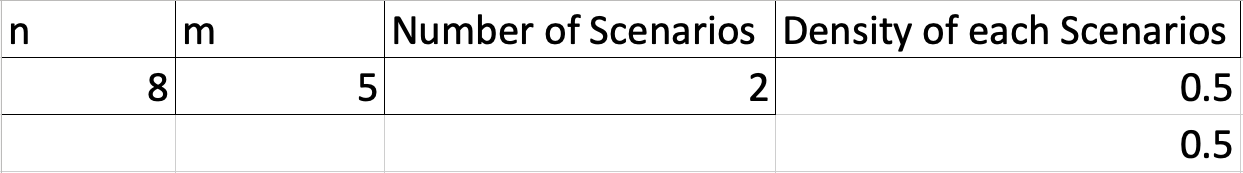
\includegraphics[width=1\textwidth]{Images/p1Input.png}
	\caption{Dữ liệu đầu vào của Problem 1}
    \end{figure}
    
    Ta sẽ tiến hành chạy chương trình bằng cách nhập câu lệnh sau lên terminal (lưu ý trước khi chạy vào chuyển terminal đến thư mục của file chương trình): \texttt{python3 p1.py} hoặc \texttt{python p1.py} tuỳ vào thiết bị chạy và các cài đặt của. Kết quả sau khi chạy chương trình 2 lần:
    \begin{figure}[h]
        \captionsetup{justification=centering}
        \centering
        \begin{subfigure}[b]{0.45\linewidth}
            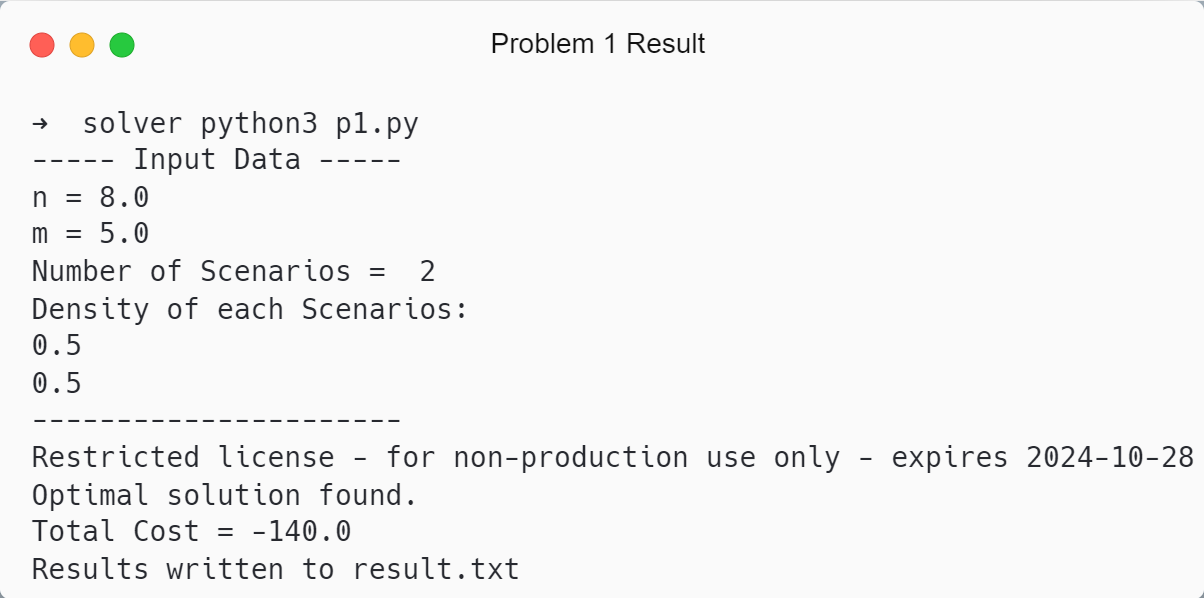
\includegraphics[width=\linewidth]{Images/result1.png}
            \caption{Lần 1}
        \end{subfigure}
        \begin{subfigure}[b]{0.45\linewidth}
            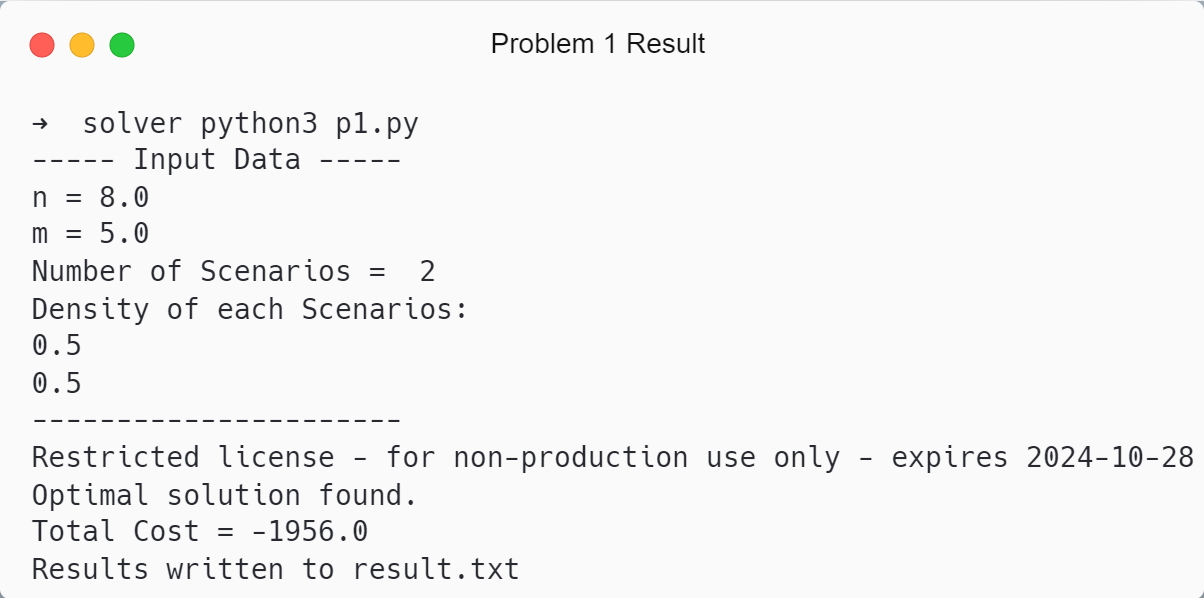
\includegraphics[width=\linewidth]{Images/carbon(2).png}
            \caption{Lần 2}
        \end{subfigure}
	\caption{Kết quả khi giải Problem 1}
    \end{figure}

    Kết quả chi tiết của từng biến sẽ được viết vào file \texttt{result.txt} (sẽ được tạo tự động khi chương trình chạy). Ta thấy được cho dù các hệ số có thay đổi ra sao thì ta vẫn có thể tìm ra kết quả tối ưu. Và đặc biệt trong 1 vài trường hợp thì kết quả tối ưu có thể ra 0.
        \subsection{Giải thích kết quả} %Fix sau
    Chúng ta sẽ giải chương trình với n=8, với trường hợp  S = 2, $p_s = 1/2$, số lượng bộ phận đặt hàng trước khi sản xuất m =5, và mô phỏng ngẫu nhiên các vector b, l, q, s và ma trận A với kich thước $n\times m$. Và cũng giả sử rằng vetor $\omega = D =(D_1,D_2,\dots , D_3)$ với mỗi $\omega_i$ với mật độ $p_i$ tuân thủ theo phân bố nhị thức (10,1/2) . Và đương nhiên chúng ta sẽ tìm được nghiệm tối ưu của bài toán. Tuy nhiên trong 1 vài trường hợp thì nghiệm tối ưu này bằng 0. Giải thích cho vấn đề này thì chúng ta cần hiểu sâu hơn về bài toán. Đây là 1 dạng bài toán về kinh tế, cho nên việc chi phí > doanh thu thì sẽ gây ra thua lỗ và công ty có thể phá sản. Cho nên với trường hợp này sau khi tính toán được chi phí > doanh thu thì cách tôt nhất để đảm bảo sự vận hành của công ty đó chính là dừng lại quá trình sản xuất để không bị thua lỗ.Vì vậy cho nên nghiệm tối ưu cho chi phí bé nhất trong trường hợp này chính là 0 vì chúng ta không sản xuất . 
    %%%%%%%%%%%%%%%%%%%%%%%%%%%%%%%%%

\section{Ứng dụng Stochastic Linear Program cho việc lập kế hoạch sơ tán trong ứng phó thiên tai}
\subsection{Giới thiệu}
Những thiên tai ảnh hưởng đến cuộc sống của con người có thể tấn công một cách bất ngờ và không có nhiều dấu hiệu từ trước để lại rất nhiều thiệt hại về cả tài sản và con người. Mục tiêu chính của ứng phó khẩn cấp là cung cấp nơi trú ẩn và hỗ trợ cho những người bị ảnh hưởng càng sớm càng tốt. Để làm được điều này, những nghiên cứu thường tập trung vào việc ứng phó khẩn cấp về cách người dân ở các khu vực an toàn có thể được hỗ trợ các nhu yếu phẩm hoặc tiếp cận các trung tâm hỗ trợ. Các nghiên cứu liên quan đến việc điều tra và lập kế hoạch sơ rán rõ ràng cho những người bị ảnh hưởng từ khu vực nguy hiểm đến khu vực an toàn. Trong bài báo cáo này tập trung vào việc lập kế hoạch về đường sơ tán cho những người bị ảnh hưởng bằng cách xây dựng một mô hình chung khi thảm hoạ xảy ra. Thiên tai là một sự cố ngoài ý muốn và không thể dự đoán trước được khi nào nó xảy ra và cũng như tác động và thiẹt hại của nó và hiển nhiên ta cũng sẽ không thể biết trước cường độ của nó. Do đó bài toán lập kể hoạch sơ tán này là một bài toán ngẫu nhiên. Nói cách khác, thiệt hại có thể xảy ra ngẫu nhiên trên một con đường và ngăn cản việc di tản đến nơi an toàn.

Với sự phát triển của internet và công nghệ thông tin hiện đại, mọi người có thể tiếp cận thông tin về hệ thống đường đi theo thời gian thực sau các sự kiện bất ngờ thông qua nhiều kênh khác nhau. Vì vậy, làm thế nào để tìm ra con đường sơ tán tối ưu cho những người bị ảnh hưởng trong điều kiện có sẵn thông tin theo thời gian thực là vấn đề được quan tâm trong bài này. 
\subsection{Model cho bài toán sơ tán}
\subsubsection{Giới thiệu các biến trong bài toán}
Để giải quyết vấn đề về việc lập kế hoạch sơ tán ta sẽ cần phải giải một bài toán Stochastic Linear Programing theo dạng min-cost flow problem với thời gian di chuyển và capacity ngẫu nhiên trên một graph $G(V,A,C,U,D)$ với $V$ là tập hợp các Node, $A$ là tập hợp các đường đi với thời gian di chuyển và capacity là ngẫu nhiên, $C$ đại diện cho thời gian di chuyển trên các đường đi thuộc A (ký hiệu là $c_{ij}$), $U$ đại diện cho capacity trên các đường đi thuộc A (ký hiệu là $u_{ij}$) và $D$ là flow tại node $i \in V$. Model cho bài toán 2-stage trên đồ thị G với stage 1 là $\sum_{(i,j)\in A} p_{ij}x_{ij}$ đại diện cho việc xác định phương án tối ưu trước khi thiên tai xảy ra. Bởi độ thiệt bởi thiên tai là một chuyện không thể đoán trước vì thế ở stage 2 ta sẽ random các giá trị và tính toán dựa trên giá trị kỳ vọng (Expected value $E$) của những lần random và stage 2 sẽ có dạng $\sum_{(i,j \in A_s)}c^s_{ij}(t)\cdot y^s_{ij}(t))$. Cụ thể các biến có thể xem ở bảng bên dưới:
\begin{center}
\begin{table}[ht!]
  \centering
  \caption{Biến quyết định}
\begin{tabular}{cl}
\hline
Decision variables & Definition \\
\hline 
$x_{i,j}$& the flow on link {i,j} \\
$y_{i,j}^s (t)$ & the flow on link {i,j} in scenario s at time t\\
\hline 
\end{tabular}
\end{table}
\end{center}

\begin{center}
\begin{table}[ht!]
  \centering
  \caption{Biến dùng trong mô hình}
\begin{tabular}{cl}
\hline
  Symbol & Definition \\
   \hline
  $V$ & the set of nodes \\
 $A$  & the set of links  \\
   $i,j$ &the index of nodes $i,j \in V$ \\
   $$(i,j)$$ & the index of directed links, $(i,j) \in A$ \\
   $s$& the index of scenario \\
   $S$& the total number of scenario \\
   $v$ & the supply value of source node \\ 
   $\tilde{T}$& the time threshold\\
   $T$ & the total number of  time intervals\\
   $u_{i,j}$ & the capacity on physical links (i,j)\\
   $u_{i,j}^s (t)$ & the capacity of link (i,j) in scenario s at time t\\
   $c_{i,j}^s (t)$ &  the travel time of link (i,j) in scenario s at time t\\
   $u_s$& the probability in scenario s\\
   \hline 
\end{tabular}
\end{table}
\end{center}


\subsubsection{Các ràng buộc của bài toán}
Stage 1:

Trong giai đoạn đầu của bài toán cần phải xác định được phương án di tản khả thi từ super-source và super-sink. Và để xác định được điều này phải đáp ứng được các ràng buộc sau đây. 

\[ \sum_{(i,j)\in A }  x_{ij} -\sum_{(j,i) \in A} x_{ji} = d_i\]

Trong đó ta có d là tham số với định nghĩa như sau
\begin{center}
$d_i=$
$\begin{cases}
&v , i=S \\
& -v, i=t\\
&0, otherwise
\end{cases}$
\end{center}

Đồng thời trong đó luồng trên mỗi đường cũng phải đáp ứng được ràng buộc sau đây:
\[ 0 \leqslant x_{ij} \leqslant \mu_{ij} , \forall (i,j) \in A\]
Một lưu ý cuối cùng rằng các ràng buộc cân bằng luồng có thể tạo ra một đường dẫn có các vòng lặp và các chuyến tham quan phụ nếu có các vòng lặp tiềm năng trong quá trình sơ tán. Để loại bỏ cấc vòng lặp trên đường sơ tán vật lí được tạo ra, link penalty $p_{ij}$ ,(i,j)$\in$ A được xem xét đến. vậy nên hàm penalty có để def là :
\[ f(\textbf{X}) = \sum _{(i,j) \in A} p_{ij} \cdot x_{ij} \text{ với } \textbf{X} := {x_{ij}}_{(i,j) \in A.}\]


Stage 2:

Để giải quyết stage 1 thì việc giải quyết được stage 2 chính là 1 điều tiên quyết. Trong stage này, những người bị ảnh hưởng bởi thiên tai sẽ nhận được các lộ trình thích ứng với thời gian sơ tán tối thiểu theo thông tin thảm họa thời gian thực.Các kế hoạch sơ tán trong các tình huống khá nhau trước ngưỡng thời gian đều gióng với priori path.Các ràng buộc ghép nối cho kế hoạch sơ tán của từng kịch bản với ngưỡng thời gian T có thể được xây dựng như sau : 
\[\sum_{t \leqslant \tilde{T} } y_{ij}^s (t) = x_{ij} , (i,j) \in A ,s = 1,2,\dots ,S \]
Ràng buộc này thể hện mối liên hệ giữa physical link và space-time arc trong kế hoạch sơ tán. Nghĩa là, nếu có các luồng lưu lượng trên liên kết $$(i,j)$$ chẳng hạn như $x_{i j} = 2$ thì luồng lưu lượng trên liên kết $$(i,j)$$ trước ngưỡng thời gian là 2 hay là $y(t) = 2$. Nói cách khác kế hoạch sơ tán trong từng kịch bản của giai đoạn 2 giống như kế hoạch sơ tán ở giai đoạn đầu.
\begin{center}
    $\begin{cases}
        & Q(Y,s) = min \sum _{(i,j) \in A_s} c_{ij}^s(t) \cdot y_{ij}^s(t) \\
        & \text{Subject to :}\\
        & \sum_{(i_t,j_{t'})\in A_s} y_{ij}^s(t) -\sum_{(j_{t'},i_t)\in A_s} y_{ij}^s(t') = d_j^s(t), \forall  \text{ } i \in V \\
        &t\in {0,1,\dots , T} , s = 1,2,\dots S\\
        & 0 \leqslant y_{i,j}^s (t) \leqslant u_{i,j}^s (t) , A (i,j) \in A,t \in {0,1,\dots , T} , s = 1,2,\dots , S \\
        & \sum_{t\leqslant \tilde{T}}  y_{i,j}^s (t) = x_{ij},(i,j) \in A, s= 1,2,\dots ,S\\
    \end{cases}$
\end{center}
Hàm mục tiêu ở trên là thời gian sơ tán tổng thể của tất cả mọi người trong scenario S. Các ràng buộc lần lượt là ràng buộc về hạn chế về cân bằng luồng và hạn chế về năng lực giao thông.Ràng buộc cuối cùng là ràng buộc ghép để đảm bảo rằng kế hoạch sơ tán đều khả thi trong thời gian $\tilde{T}$ giống với kế hoạch nghiệm ở giai đoạn 1.
\subsubsection{Model hoàn chỉnh}
Kết hợp những thông tin ở trên. Ta có thể tổng hợp các ràng buộc lại và tổng hợp lại thành 1 model chung nhất cho bài toán như sau.
\begin{center}
\textbf{Model = }
$\begin{cases}
&\min \sum_{(i,j)\in A} p_{ij}x_{ij} + \sum_{s=1}^{S}(\mu_s \cdot \sum_{(i,j \in A_s)}c^s_{ij}(t)\cdot y^s_{ij}(t)) \\
&\text{Subject to} \\
& \sum_{(i,j)\in A} x_{ij} - \sum_{(j,i)\in A}x_{ji} = d_i, \forall i\in V \\
&0\leqslant x_{ij} \leqslant u_{ij}, \forall (i,j) \in A \\
& \sum_{(i_t,j_{t'})\in A_s} y_{ij}^s(t) -\sum_{(j_{t'},i_t)\in A_s} y_{ij}^s(t') = d_j^s(t), \forall  \text{ } i \in V \\
&t\in {0,1,\dots , T} , s = 1,2,\dots S\\
& 0 \leqslant y_{i,j}^s (t) \leqslant u_{i,j}^s (t) , A (i,j) \in A,t \in {0,1,\dots , T} , s = 1,2,\dots , S \\
& \sum_{t\leqslant \tilde{T}}  y_{i,j}^s (t) = x_{ij},(i,j) \in A, s= 1,2,\dots ,S

\end{cases}$
\end{center}

Model trên về cơ bản một bài toán quy hoạch tuyến tính với 2 loại biến quyết định là $\textbf{X}:={x_{ij}}_{(i,j)\in A}$ và $\textbf{Y}:={y_{ij}^s (t)}_{(i,j)\in A,t \in {0,1,\dots , T},s=1,2,\dots ,S}$. Trong model này có những ràng buộc phức tạp nên không thể giải quyết trong thời gian tuyến tính. Ta sẽ sử dụng phương pháp Lagrangian Relaxtion để đơn giản hóa model ban đầu thành 2 model nhỏ hơn để có thể giải quyết hiệu quả bằng các thuật toán, nơi mà giá trị sau khi giải quyết 2 bài toán trên là lower bound và upper bound của bài toán. Cụ thể 2 model được tách ra đó chính là 2 bài toán \textbf{Min-Cost-Flow} và \textbf{Time-Dependent}. 
\subsection {Đơn giản hóa mô hình}
Từ mô hình ban đầu có thể thấy rằng ràng buộc kép $\sum_{t \leqslant \tilde{T} } y_{ij}^s (t) = x_{ij} , (i,j) \in A ,s = 1,2,\dots ,S $ là một điều kiện cứng. Do đó, chúng ta sẽ sử dụng hệ số nhân Lagrangian $(t),(i,j)\in A,s= 1,2,\dots ,S,t \leqslant \tilde{T}  $ để lới lỏng ràng buộc này thành như sau:

\[\sum_{s=1}^S \sum _{t \leqslant \tilde{T}} \sum_{(i,j)\in A} \alpha _{i,j}^s (t)(y_{ij}^s (t) - x_{ij})  \]


Sau khi dùng Lagrangian để đơn giản model bài toán thì model mới sẽ như sau:

\begin{center}
$\begin{cases}
 &min \sum_{i,j \in A} P_{ij} X_{ij} + \sum_{s=1}^s( \mu \cdot \sum_{(i,j)\in A_s} c_{ij}^s(t) \cdot y_{ij}^s (t)) + \\
 &\sum_{s=1}^s \sum_{t \leqslant \tilde{T}} \sum_{(i,j) \in A} \alpha _{ij}^s (t) (y_{ij}^s (t) -x_{ij})\\
 & \text{ subject to :} \\
 & \sum_{(i,j) \in A} x_{(ij)} - \sum _{(ji)\in A} x_{ij} = d_i, \forall \text{ i}\in V\\
 & 0 \leqslant x_{ij} \leqslant \mu_{ij}, \forall \text{ (i,j)} \in A \\
 & \sum_{(i_t,j_{t'})\in A_s} y_{ij}^s (t) - \sum_{(i_t,j_{t'})\in A_s} y_{ij}^s (t') = d_i^s (t) , \forall \text{ i} \in V\\
 & t\in {0,1,\dots , T} , s= 1,2,\dots S \\
 & 0 \leqslant y_{ij}^s (t) \leqslant \mu_{ij} ^ s (t), \forall \text{ (i,j)} \in A, t \in {0,1,\dots, T}, s=1,2,\dots , S \\
\end{cases}$
\end{center}
 Có 1 điều cần lưu ý là 2 biến X và Y có thể tách biệt với nhau trong model ở trên. Nghĩa là bằng các này thì model thoải mái được tách ra thành 2 bài toán con đó là 2 bài toán \textbf{Min-Cost-Flow} và \textbf{Time-Dependent}. Với bài toán đầu tiên thì nó có thể được coi là bài toán tối ưu chi phí với model của nó được đưa ra với dạng như sau :
 \begin{center}
$ \begin{cases}
&\text{minSP1}( \alpha) = \sum_{(i,j)\in A} (P_{ij} - \sum_{s=1}^{S} \sum_{t \leqslant \tilde{T}} \alpha_{ij}^s (t))_{x_{ij}}\\
& \text{subject to.}\\
& \sum_{(i,j)\in A} x_{ij} - \sum_{(j,i) \in A} x_{ij} = d_j , \forall \text{ i} \in V \\
& 0 \leqslant x_{ij} \leqslant u_{ij}, \forall \text { (i,j)} \in A\\
\end{cases}$
\end{center}


Với bài toán thứ 2 liên quan đến các biến quyết định Y và giá trị mục tiêu của bài toán với Model được biểu diễn như sau:
  \begin{center}
$ \begin{cases}
& minSP2(\alpha) = \sum_{s=1}^s \sum_{(i,j)\in A}(\sum_{t\in(0,1,\dots , T)} \mu_s \cdot c_{ij}^s (t) + \sum_{t \leqslant \tilde{T}} \alpha_{ij}^s (t) ) y_{ij}^s (t) \\
& \text{subject to} \\
& \sum_{(i_t,j_{t'})\in A_s} y_{ij}^s (t) - \sum_{(i_t,j_{t'})\in A_s} y_{ij}^s (t') = d_i^s (t) , \forall \text{ i} \in V\\
 & t\in {0,1,\dots , T} , s= 1,2,\dots S \\
 & 0 \leqslant y_{ij}^s (t) \leqslant \mu_{ij} ^ s (t), \forall \text{ (i,j)} \in A, t \in {0,1,\dots, T}, s=1,2,\dots , S \\
\end{cases}$
\end{center}
 Và bây giờ chúng ta cùng tiến tới việc xây dựng chương trình giải của bài toán.
\subsection{Xây dựng chương trình giải}
\subsubsection{SubProblem 1}
Ở nội dung của bài báo cáo này ta chỉ xét đến việc giải bài toán min-cost flow nghĩa là chỉ tập trung vào việc giải SubProblem 1. Gọi $g_{ij} := p_{ij} - \sum_{s=1}^S \sum_{t\leq \tilde{T}} \alpha^{s}_{ij}(t)$ là chi phí của mỗi đường đi SubProblem 1 sẽ trở thành như sau:
\begin{center}
$ \begin{cases}
&\text{minSP1}( \alpha) = \sum_{(i,j)\in A} g_{ij}\cdot x_{ij}\\
& \text{subject to.}\\
& \sum_{(i,j)\in A} x_{ij} - \sum_{(j,i) \in A} x_{ij} = d_j , \forall \text{ i} \in V \\
& 0 \leqslant x_{ij} \leqslant u_{ij}, \forall \text { (i,j)} \in A
    
\end{cases}$
\end{center}
\subsubsection{Algorithm 1}
Algorithm 1 là một thuật toán dùng để giải quyết vấn đề min-cost flow mà ta quan tâm, thuật toán có thể hiểu đơn giản như sau (tham khảo tài liệu thao khảo để hiểu rõ hơn): 
\begin{enumerate}
\item Lấy $x$ là một luồng (flow) khả thi giữa các đường đi và nó có chi phí thấp nhất trong những luồng khả thi.
\item Thuật toán kết thúc nếu giá trị luồng của $x$ đạt tới giá trị $v$ hoặc không có đường đi thoã mãn; nếu không, đường gắn nhất với luồng tối đa trong đường đi có chi phí tối thiểu trong hệ thống đường được tính toán bằng thuật toán, sau đó đi đến Bước 3.
\item Tăng các luồng nếu nó chưa vượt quá giá trị $v$, nếu không trở lại bước 2.
\end{enumerate}

Để tìm được đường đi ngắn nhất ta có nhiều thuật toán với độ phức tạp khác nhau, ở chương trình giải mà ta xây dựng bằng python dưa theo Algorithm 1 ta sẽ chọn thuật toán Bellman-Ford. Mã giả cho chương trình giải như sau:

\begin{algorithm}
\caption{Successive Shortest Path}
\KwData{Graph with cost, capacity, source and target}
\KwResult{Min-cost}
min-cost $\gets$ 0

Initialize flow x
\While{$True$}{
    Find minimum cost path
    
    $path$ $\gets$ minimum cost path
    
    \If{path is None}{
      Break
    }
    
    Find the maximum flow that can go through $path$
    
    Increase the flow among the $path$
    
    Update min-cost
}
Return min-cost
\end{algorithm}

Đây chỉ là mã giả cho thuật toán chính trong chương trình sẽ còn các hàm phụ để giúp chương trình có thể hoạt động cũng như đưa ra kết quả một cách trực quan.


\subsubsection{Chương trình giải}
Dựa vào mã giả trên ta sẽ viết chương trình giải, chương trình được viết bằng ngôn ngữ python và được viết ở Google Colab có thể truy cập từ: \href{github.com/toanhac/mm231solver}{github.com/toanhac/mm231solver}. Có thể chạy trực tiếp để xem kết quả hoặc xem qua phần kết quả được trình bài ở phần sau.

Để kiểm tra xem liệu chương trình của có hoạt động chính xác hay không ta sẽ kiểm tra kết quả do chương trình giải ra và kết quả được một chương trình khác được xây dựng bởi google (developers.google.com/optimization/flow/mincostflow). Dưới đây là kết quả của hai chương trình với cùng một dữ liệu đầu vào như sau:

\begin{center}
\begin{tabular}{ccc}
    Arc & Capacity & Cost \\
    0 -> 1 & 15 & 4 \\
    0 -> 2 & 8 & 4 \\
    1 -> 2 & 20 & 2 \\
    1 -> 3 & 4 & 2 \\
    1 -> 4 & 10 & 6 \\
    2 -> 3 & 15 & 1 \\
    2 -> 4 & 4 & 3 \\
    3 -> 4 & 20 & 2 \\
    4 -> 2 & 5 & 3 \\
\end{tabular}
\end{center}

Đây là kết quả của chương trình được xây dựng bởi google trả về:
\begin{center}
Minimum cost: 150 \\
\begin{tabular}{cc}
    Arc & Flow \\
    0 -> 1 & 12 \\
    0 -> 2 & 8 \\
    1 -> 2 & 8 \\
    1 -> 3 & 4 \\
    1 -> 4 & 0 \\
    2 -> 3 & 12 \\
    2 -> 4 & 4 \\
    3 -> 4 & 11 \\
    4 -> 2 & 0 \\
\end{tabular}
\end{center}
Còn đây là kết quả chương trình mà ta xây dựng trả về: 
\begin{itemize}
\item Flow: {('0', '1'): 12, ('0', '2'): 8, ('3', '4'): 11, ('4', '2'): 0, ('1', '2'): 8, ('1', '3'): 4, ('1', '4'): 0, ('2', '3'): 12, ('2', '4'): 4}
\item Minimum cost: 150
\end{itemize}

Ta có thể chương trình của ta đã hoạt động chính xác với những gì mà ta mong muốn. Giờ đây ta sẽ tiến hành chạy nó trên một đồ thị lớn hơn để xem xét về độ hiểu quả của Algorithm 1.
\subsection{Thử nghiệm Algorihtm 1}
\subsubsection{Thiết kế thử nghiệm}
Thử nghiệm này sẽ chạy trên một đồ thị gồm 50 node, 85 links (hình bên dưới) và sẽ có 50 xe cần di chuyển.

\begin{figure}[h]
	\captionsetup{justification=centering}
	\centering
	
\begin{tikzpicture}
\foreach \i in {1,...,10} {
    \foreach \j in {0,...,4} {
        \node[draw,circle, minimum size=0.7cm, inner sep=0pt,] (\the\numexpr\j*10+\i) at (\i*1.5,-\j*1.5) {\the\numexpr\j*10+\i};
    }
}

\foreach \i in {1,...,9} {
    \foreach \j in {0,...,3} {
        \draw[decoration={markings,mark=at position 1 with
    {\arrow[scale=2,>=stealth]{>}}},postaction={decorate}] (\the\numexpr\j*10+\i) -- (\the\numexpr\j*10+\i+1);
        \draw[decoration={markings,mark=at position 1 with
    {\arrow[scale=2,>=stealth]{>}}},postaction={decorate}] (\the\numexpr(\j*10+\i)) -- (\the\numexpr\j*10+\i+10);
    }
}
\draw[decoration={markings,mark=at position 1 with
    {\arrow[scale=2,>=stealth]{>}}},postaction={decorate}] (41) -- (42);
\draw[decoration={markings,mark=at position 1 with
    {\arrow[scale=2,>=stealth]{>}}},postaction={decorate}] (42) -- (43);
\draw[decoration={markings,mark=at position 1 with
    {\arrow[scale=2,>=stealth]{>}}},postaction={decorate}] (43) -- (44);
\draw[decoration={markings,mark=at position 1 with
    {\arrow[scale=2,>=stealth]{>}}},postaction={decorate}] (44) -- (45);
\draw[decoration={markings,mark=at position 1 with
    {\arrow[scale=2,>=stealth]{>}}},postaction={decorate}] (45) -- (46);
\draw[decoration={markings,mark=at position 1 with
    {\arrow[scale=2,>=stealth]{>}}},postaction={decorate}] (46) -- (47);
\draw[decoration={markings,mark=at position 1 with
    {\arrow[scale=2,>=stealth]{>}}},postaction={decorate}] (47) -- (48);
\draw[decoration={markings,mark=at position 1 with
    {\arrow[scale=2,>=stealth]{>}}},postaction={decorate}] (48) -- (49);
    \draw[decoration={markings,mark=at position 1 with
    {\arrow[scale=2,>=stealth]{>}}},postaction={decorate}] (49) -- (50);
\draw[decoration={markings,mark=at position 1 with
    {\arrow[scale=2,>=stealth]{>}}},postaction={decorate}] (10) -- (20);
\draw[decoration={markings,mark=at position 1 with
    {\arrow[scale=2,>=stealth]{>}}},postaction={decorate}] (20) -- (30);
\draw[decoration={markings,mark=at position 1 with
    {\arrow[scale=2,>=stealth]{>}}},postaction={decorate}] (30) -- (40);
\draw[decoration={markings,mark=at position 1 with
    {\arrow[scale=2,>=stealth]{>}}},postaction={decorate}] (40) -- (50);
\end{tikzpicture}

	\caption{Tesing network}
\end{figure}
    

\subsubsection{Thử nghiệm thời gian chạy so với chương trình của Gurobi} 
Capacity và Cost trên mỗi link sẽ là như nhau ở 2 cái chương trình. Hệ thống được sử dụng để thử nghiệm là: 
\begin{itemize}
\item CPU model: Intel(R) Core(TM) i5-5350U CPU @ 1.80GHz
\item Thread count: 2 physical cores, 4 logical processors, using up to 4 threads
\end{itemize}
Kết quả sau một số lần thử nghiệm được trình bài ở bảng bên dưới (thời gian trung bình).
\begin{center}
\begin{table}[h!]
  \centering
  \caption{Kết quả khi so với chương trình của Gurobi}
  \begin{tabular}{cccc}
    \hline
    OD pair & Số lần chạy & Gurobi Run Time & Our Run Time \\
    \hline
    $1\rightarrow 37$ & 5 & 1,216(s) & 2,286(s)\\
    $1,7 \rightarrow 36, 47$& 5 & 1,193(s) & 2,347(s)\\
    $2,7,8\rightarrow 37,33,50$ & 5 & 1,120(s) & 2,533(s)\\
    $1,2,3,4 \rightarrow 47,48,49,50$& 5 & 1,133(s) & 2,483(s)\\
    $1,2,3,4 \rightarrow 47,48,49$& 5 & 1,050(s) & 2,497(s)\\
    \hline
  \end{tabular}
\end{table}
\end{center}
Qua kết quả trên ta có thể thấy chương trình của ta chạy chậm hơn chương trình của Gurobi khá nhiều và với kết quả này ta có thể nhận xét rằng chương trình của ta chưa phải chương trình có thuật toán tốt nhất để giải bài toán min-cost flow và chương trình của ta cũng chưa tối ưu được chương trình. Để có thể xem rõ hơn về thời gian của chương trình ta sẽ tiến hành chạy thử nghiệm với capacity và cost của mỗi like được sinh ngẫu tạo cho chương trình nhiều khả năng xảy ra của đường đi hơn. Kết quả được ghi vào bảng bên dưới:
\begin{center}
\begin{table}[h!]
  \centering
  \caption{Kết quả khi chạy với các giá trị random}
\begin{tabular}{cccc}
    \hline
    OD pair & Số thứ tự của lần chạy & Run Time \\
    \hline
    $1\rightarrow 37$ & 1 &  2,33(s)\\
    $1\rightarrow 37$& 2 & 2,36(s)\\
    $1\rightarrow 37$ & 3 &  2,23(s)\\
    $1,2,3,4,5,6 \rightarrow 46,47,48,49,50$& 1 & 2,92(s)\\
    $1,2,3,4,5,6 \rightarrow 46,47,48,49,50$& 2 & 2,71(s)\\
    $1,2,3,4,5,6 \rightarrow 46,47,48,49,50$& 3 & 2,75(s)\\
    $20,15,40,25 \rightarrow 45,30,50$& 1 & 2,37(s)\\
    $20,15,40,25 \rightarrow 45,30,50$& 2 & 2,47(s)\\
    $20,15,40,25 \rightarrow 45,30,50$& 3 & 2,30(s)\\
    \hline
  \end{tabular}
\end{table}
\end{center}
Algorithm 1 chính xác về mặt kết quả nhưng về mặt thời gian thì giải thuật này có thời gian thực thi chậm hơn tương đối so với các giải thuật khác. Đây cũng có thể một phần do lỗi của chương trình chưa được tối ưu. Trong tương lai nếu có thể cải thiện code để cải thiện thời gian chạy của chương trình thì đây sẽ là một giải thuật khá hiệu quả và sẽ đóng góp rất lớn trong quá trình quyết bài toán di tản, một bài toán rất cấp thiết.

\begin{thebibliography}{80}

\bibitem{bib1}
A. Shapiro, D. Dentcheva, and A. Ruszczynski, Lectures on stochastic programming: modeling and theory. SIAM, 2021.

\bibitem{bib2}
L. Wang, “A two-stage stochastic programming framework for evacuation planning in disaster responses,” Computers $\&$ Industrial Engineering, vol. 145, p. 106458, 2020.

\bibitem{bib3}
Gurobi Optimization, LLC, "Gurobi: The Leader in Decision Intelligence," 2023. [Online]. Available: https://www.gurobi.com/.

\bibitem{bib4}
Google Developers, "Minimum Cost Flow," 2023. [Online]. Available: https://developers.google.com/optimization/flow/mincostflow.

\end{thebibliography}
\end{document}

